A modelagem matemática utilizada para um quadrotor neste trabalho foi a proposta por \citeonline{Balas2007}, devido à sua abordagem completa incluindo diferentes estágios: desacoplamento das entradas, dinâmicas dos rotores e modelagem do quadrotor em si. A estrutura utilizada nesta modelagem é mostrada na \autoref{fig:Balas2007_diagram_blocos_drone_abordagem_engenharia}.

\begin{figure}[!htb]
    \centering
    \caption{Diagrama de blocos do sistema de representação de um quadricóptero}
    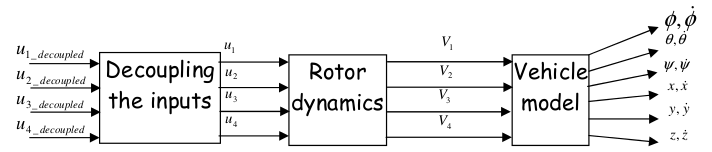
\includegraphics[width=1\textwidth]{./04-figuras/Balas2007_diagram_blocos_drone_abordagem_engenharia}
    \fonte{\citeonline[p.~58]{Balas2007}}
    \label{fig:Balas2007_diagram_blocos_drone_abordagem_engenharia}
\end{figure}

Nesta estrutura, $u_1$ representa o empuxo total sobre o quadricóptero, $u_2$ representa o momento de \textit{roll} (em torno do eixo $x$), $u_3$ representa o momento de \textit{pitch} (em torno do eixo $y$) e $u_4$ representa o momento de \textit{yaw} (em torno do eixo $z$). $u_{2\textunderscore decoupled}$, $u_{3\textunderscore decoupled}$ e $u_{4\textunderscore decoupled}$ são combinações de $u_2$, $u_3$ e $u_4$ de tal forma que as entradas $u_{2\textunderscore decoupled}$, $u_{3\textunderscore decoupled}$ e $u_{4\textunderscore decoupled}$ tenham as mesmas direções que os ângulos de Euler, $\phi$, $\theta$ e $\psi$, respectivamente. A relação entre estas entradas é dada, em \cite[p.~49]{Balas2007} por:
\[
	\begin{bmatrix}
		u'_{2} \\
		u'_{3} \\
		u'_{4}
	\end{bmatrix} = 
	\begin{bmatrix}
		cos_{\psi_{0}} & sen_{\psi_{0}}cos_{\phi_{0}}\frac{I_{xx}}{I_{yy}} & 
		0 \\
		
		-sen_{\psi_{0}}\frac{I_{yy}}{I_{xx}} &
		cos_{\psi_{0}}cos_{\phi_{0}} &
		0 \\
		
		0 &
		-sen_{\phi_{0}}\frac{I_{zz}}{I_{yy}} &
		1
	\end{bmatrix}
	\begin{bmatrix}
		u'_{2\textunderscore decoupled} \\
		u'_{3\textunderscore decoupled} \\
		u'_{4\textunderscore decoupled}
	\end{bmatrix}
\]

$I_{xx}$, $I_{yy}$ e $I_{zz}$ representam o momento de inércia do quadricóptero ao longo dos eixos $x$, $y$ e $z$, respectivamente.

Na \autoref{fig:Balas2007_diagram_blocos_drone_abordagem_engenharia}, o primeiro bloco, referente ao desacoplamento das entradas, atua justamente convertendo as entradas $u_{1\textunderscore decoupled}$ $u_{2\textunderscore decoupled}$, $u_{3\textunderscore decoupled}$ e $u_{4\textunderscore decoupled}$ de forma a se obter $u_1$, $u_2$, $u_3$ e $u_4$ para que, no bloco seguinte, de dinâmicas dos rotores, as entradas sejam, de forma isolada, o empuxo total sobre o quadricóptero e os momentos de \textit{roll}, \textit{pitch} e \textit{yaw}. Neste bloco, estabelece-se uma relação entre essas quatro entradas e a tensão que deve ser aplicada a cada um dos rotores, $V_1$, $V_2$, $V_3$ e $V_4$.

Por fim, o último bloco, referente à \textit{Modelagem do Quadrotor}, apresenta o estado do quadrotor, fornecendo, como saída, os ângulos de \textit{roll}, \textit{pitch} e \textit{yaw}, a posição do quadrotor nos eixos $x$, $y$ e $z$ tal como a taxa de variação de cada uma destes ângulos e posições.

\subsection{Modelagem Matemática}
\label{subsec:sistemas-quadcopter-mathematical-model}

Em \cite{Balas2007}, a modelagem do quadricóptero foi feita em três partes: uma sendo referente ao empuxo vertical; uma segunda, aos momentos de \textit{roll} e \textit{pitch}; e uma terceira, ao momento de \textit{yaw}.

%Assumindo um quadricóptero com massa $m$ igual a 2,354 g e uma aceleração $g$ igual a 9,81 N.
A função de transferência obtida por \citeonline[p.~20]{Balas2007} para representar o empuxo vertical gerado pelos quatro rotores do quadrotor foi:
\begin{equation}
H(s) = \frac{2,105s-0,0425}{0,4895s^2+1,873s+1} N/V
\end{equation}

Já a função de transferência obtida para representar os momentos de \textit{roll} e de \textit{pitch} foi:
\begin{equation}
H(s) = l\frac{1,155s}{0,8696s^2+0,401s+1} Nm/V
\end{equation}

Por fim, a função de transferência obtida para representar o momento de \textit{yaw} foi:
\begin{equation}
H(s) = \frac{0,045}{0,314s+1} Nm/V
\end{equation}

\subsection{Representação no Espaço de Estados}
\label{subsec:sistemas-quadcopter-state-spaces}

Como mostrado em \cite[p.~63]{Balas2007}, o sistema modelado pode ser representado da seguinte forma no espaço de estados.
\begin{align} \label{eq:space_state_equation_quadcopter}
	\dot{x} &= Ax + Bu \nonumber \\
	y		&= Cx + Du
\end{align}

Com o vetor de estados $X$ sendo dado por:
\begin{equation*}
X=
\left[ \begin{array}{@{}*{12}{c}@{}}
     x & y & z & \dot{x} & \dot{y} & \dot{z} & \phi & \theta & \psi & \dot{\phi} & \dot{\theta} & \dot{\psi}\\
\end{array} \right]^T
\end{equation*}

O vetor de entrada $U$ sendo dado por:
\[ 
	U =
	\begin{bmatrix}
		u_1 & 
		u_{2\textunderscore decoupled} &
		u_{3\textunderscore decoupled} &
		u_{4\textunderscore decoupled}
	\end{bmatrix}^T
\]

As matriz A, B, C e D sendo definida como:
\begin{equation*}
A =
\left[ \begin{array}{@{}*{12}{c}@{}}
     0 & 0 & 0 & 1 & 0 & 0 & 0 & 0  & 0 & 0 & 0 & 0 \\
     0 & 0 & 0 & 0 & 1 & 0 & 0 & 0  & 0 & 0 & 0 & 0 \\
     0 & 0 & 0 & 0 & 0 & 1 & 0 & 0  & 0 & 0 & 0 & 0 \\
     0 & 0 & 0 & 0 & 0 & 0 & 0 & -g & 0 & 0 & 0 & 0 \\
     0 & 0 & 0 & 0 & 0 & 0 & g & 0  & 0 & 0 & 0 & 0 \\
     0 & 0 & 0 & 0 & 0 & 0 & 0 & 0  & 0 & 0 & 0 & 0 \\
     0 & 0 & 0 & 0 & 0 & 0 & 0 & 0  & 0 & 1 & 0 & 0 \\
     0 & 0 & 0 & 0 & 0 & 0 & 0 & 0  & 0 & 0 & 1 & 0 \\
     0 & 0 & 0 & 0 & 0 & 0 & 0 & 0  & 0 & 0 & 0 & 1 \\
     0 & 0 & 0 & 0 & 0 & 0 & 0 & 0  & 0 & 0 & 0 & 0 \\
     0 & 0 & 0 & 0 & 0 & 0 & 0 & 0  & 0 & 0 & 0 & 0 \\
     0 & 0 & 0 & 0 & 0 & 0 & 0 & 0  & 0 & 0 & 0 & 0 \\
\end{array}\right]
\end{equation*}

\begin{equation*}
B =
\left[\begin{array}{@{}*{4}{c}@{}}
	0 & 0 & 0 & 0 \\
	0 & 0 & 0 & 0 \\
	0 & 0 & 0 & 0 \\
	0 & 0 & 0 & 0 \\
	0 & 0 & 0 & 0 \\
	-1/m & 0 & 0 & 0 \\
	0 & 0 & 0 & 0 \\
	0 & 0 & 0 & 0 \\
	0 & 0 & 0 & 0 \\
	0 & cos(\psi)/I_{xx} & -sen(\psi)/I_{yy} & 0 \\
	0 & sen(\psi)/(cos(\phi)I_{xx}) & cos(\psi)/(cos(\phi)I_{yy}) & 0\\
	0 & sin(\psi)tan(\phi)/I_{xx} & cos(\psi)*tan(\phi)/I_{yy} & 1/I_{zz} \\
\end{array}\right]
\end{equation*}

\begin{equation*}
C =
\left[ \begin{array}{@{}*{12}{c}@{}}
	1 & 0 & 0 & 0 & 0 & 0 & 0 & 0 & 0 & 0 & 0 & 0 \\
	0 & 1 & 0 & 0 & 0 & 0 & 0 & 0 & 0 & 0 & 0 & 0 \\
	0 & 0 & 1 & 0 & 0 & 0 & 0 & 0 & 0 & 0 & 0 & 0 \\
	0 & 0 & 0 & 1 & 0 & 0 & 0 & 0 & 0 & 0 & 0 & 0 \\
	0 & 0 & 0 & 0 & 1 & 0 & 0 & 0 & 0 & 0 & 0 & 0 \\
	0 & 0 & 0 & 0 & 0 & 1 & 0 & 0 & 0 & 0 & 0 & 0 \\
	0 & 0 & 0 & 0 & 0 & 0 & 1 & 0 & 0 & 0 & 0 & 0 \\
	0 & 0 & 0 & 0 & 0 & 0 & 0 & 1 & 0 & 0 & 0 & 0 \\
	0 & 0 & 0 & 0 & 0 & 0 & 0 & 0 & 1 & 0 & 0 & 0 \\
	0 & 0 & 0 & 0 & 0 & 0 & 0 & 0 & 0 & 1 & 0 & 0 \\
	0 & 0 & 0 & 0 & 0 & 0 & 0 & 0 & 0 & 0 & 1 & 0 \\
	0 & 0 & 0 & 0 & 0 & 0 & 0 & 0 & 0 & 0 & 0 & 1 \\
\end{array}\right]
\end{equation*}

\begin{equation*}
D =
\left[\begin{array}{@{}*{4}{c}@{}}
	0 & 0 & 0 & 0 \\
	0 & 0 & 0 & 0 \\
	0 & 0 & 0 & 0 \\
	0 & 0 & 0 & 0 \\
	0 & 0 & 0 & 0 \\
	0 & 0 & 0 & 0 \\
	0 & 0 & 0 & 0 \\
	0 & 0 & 0 & 0 \\
	0 & 0 & 0 & 0 \\
	0 & 0 & 0 & 0 \\
	0 & 0 & 0 & 0 \\
	0 & 0 & 0 & 0 \\
\end{array}\right]
\end{equation*}

em que $g$ é a gravidade, $m$, a massa do quadrotor e os ângulos $\phi$, $\theta$ e $\psi$ representam os ângulos em torno dos eixos $x$, $y$ e $z$ respectivamente. Além disto, $I_{xx}$, $I_{yy}$ e $I_{zz}$ representam o momento de inércia do quadricóptero ao longo destes mesmos eixos.

\subsection{Experimentos Realizados}
\label{subsec:metodolgoia-quadcopter-experimentos}

Foi utilizado o algoritmo proposto em \citeonline[p.~118]{Balas2007}, que implementa a modelagem computacional descrita,  para simular as dinâmicas de um \textit{quadrotor}. Este algoritmo é mostrado no Apêndice \ref{chap:apendicex-quadcopter-modelagem}. 

A partir desta modelagem, devido ao fato de haver um bloco de desacoplamento das entradas, pôde-se obter, para cada saída, uma relação direta com apenas uma das entradas. Desta forma, num primeiro momento obtiveram-se as funções de transferência que representam estas relações. 

Uma vez definidas as funções de transferência parciais, foi criado um modelo no \textit{Simulink} para representar, num único bloco, todos os estágios da modelagem do drone: desacoplamento das entradas, dinâmicas do rotor e modelo do veículo, como apresentado na \autoref{fig:Balas2007_diagram_blocos_drone_abordagem_engenharia}. Foram feitas quatro simulações sobre este bloco em malha aberta para que se pudesse analisar graficamente as relações entre as entradas e saídas do sistema: em cada simulação, um sinal em degrau foi aplicado a uma das entradas e todas as saídas foram analisadas.

A partir das análises feitas, utilizando o \textit{Fuzzy Logic Toolbox} do MATLAB\textregistered, foram construídos três controladores Fuzzy Mamdani: um para estabilizar a atitude em torno do eixo x (ângulo $\phi$); outro para estabilizá-la em torno do eixo y (ângulo $\theta$); e um terceiro para estabilizar a altitude do motor (eixo z). O foco dos dois controladores de atitude é fazer com que, após sofrer algum tipo de distúrbio, o quadrotor seja capaz de retornar à posição horizontal. Já o foco do controlador de altitude e permitir que o quadrotor, após sofrer alguma perturbação, possa retornar à altitude em que estava antes desta perturbação ocorrer.

Feito isto, foram desenvolvidos três controladores Neuro-Fuzzy, um referente a cada um dos controladores Fuzzy desenvolvidos. Para tanto, primeiramente foi desenvolvido um controlador Fuzzy Sugeno a partir de cada um dos Mamdani. Para tanto, utilizou-se a seguinte sequência de comandos:
\begin{lstlisting}
	mamFIS = readfis('mam-filename.fis')
	sugFIS = mam2sug(mamFIS)
	writefis(sugFIS,'sug-filename.fis')
\end{lstlisting}

Na linha 1, lê-se o arquivo {\ttfamily .fis} com a estrutura do controlador Fuzzy Mamdani desenvolvido e o salva na variável {\ttfamily mamFIS}. Na linha 2 esta estrutura Mamdani é convertida para o tipo Sugeno e é salva na variável {\ttfamily sugFIS}. Por fim, na linha 3 a estrutura Sugeno é salva num novo arquivo {\ttfamily .fis}.

Após a criação dos controladores Fuzzy Sugeno, foram criados controladores Neuro-Fuzzy a partir deles. Para tanto, utilizou-se a ferramenta \textit{Neuro-Fuzzy Designer} do MATLAB para treinar as redes e validar seus respectivos treinamentos. O treinamento de cada uma das redes foi feito utilizando dados obtidos a partir dos controladores Fuzzy Mamdani.

Por fim, foram feitos testes comparando os controladores Fuzzy e Neuro-Fuzzy, para verificar se a capacidade de aprendizado e as generalizações implementadas por estes últimos são suficientes para torná-los mais eficientes do que os Fuzzy.